\documentclass[12pt,a4paper]{article}


% ------------------------------------------------------------------------
% Packages
% ------------------------------------------------------------------------
\usepackage[body={7.2in, 10in},left=0.8in,right=0.8in]{geometry}
\usepackage{amsmath,amssymb,amsfonts,graphicx,amsthm,nicefrac,mathtools, verbatim}
\usepackage{amsmath,amssymb,amsthm}
\usepackage{enumitem}
\usepackage[numbers]{natbib}
\usepackage{hyperref}
\usepackage{breqn}
\usepackage{xcolor}
\usepackage{fancyhdr}
\usepackage{float}
\usepackage{multirow}
\usepackage{url}
\usepackage{minted}

\hypersetup{
    colorlinks,
    linkcolor={red!50!black},
    citecolor={blue!50!black},
    urlcolor={blue!80!black}
}

%% If you want to define a new command, you can do it like this:
\newcommand{\Q}{\mathbb{Q}}
\newcommand{\R}{\mathbb{R}}
\newcommand{\Z}{\mathbb{Z}}
\newcommand{\C}{\mathbb{C}}
\newcommand{\E}{\mathbb{E}}
\newcommand{\V}{\mathbb{V}}



\begin{document}
% ------------------------------------------------------------------------
% Course info
% ------------------------------------------------------------------------
\begin{center}
  \textsc{ERG3020 Course Project - Twitter} \\
  CUHK-SZ, Apr 22, 2018
  \\[\baselineskip]

  % ------------------------------------------------------------------------
  % Problem set info.   Remember to change the problem set number and student name!
  % ------------------------------------------------------------------------
  \textbf{\underline{Course Project}}
\end{center}

\noindent\textbf{Student Name:}  Piao Chuxin, Ye Xiaoxing

\noindent\textbf{Student ID:}  115010058, 115010270

\noindent\hrulefill

\tableofcontents

\newpage

\section{Abstract}

  Twitter is a great firehouse of real-time information. Using the data from twitter, people can gain information such as political leaning and other tendencies. Through the classification process of the data before the election day, the more competitive candidate with a higher approval rating can be obtained.

\section{Introduction}

  American President Election is one of the catchiest affairs all over the world. To predict the candidate with higher approval rate beforehand, social networks can be effective in obtaining the political leaning of citizens in the United States.

  Twitter is one of the influential social networks that can be used in predicting the political leaning of people who use twitter. Having downloaded the data of one day from the twitter website, the emotion scores have been computed, represented by a number from -1 to 1, in which 1 represents the positive emotion while -1 represents the negative emotions. After obtaining the score of emotion, the keywords which could represent different candidate have been searched. For example, ‘Trump’ or ‘Donald’ could represent Donald Trump, and ‘Hillary’ or ‘Clinton’ could represent Hillary Clinton. Compared the twitter score which contains different key words to the average emotional score of all the twitter score, the rough political leaning of different candidates can be obtained.

  To tell the political leaning of people, we use sentiment analysis. Sentiment Analysis, sometimes known as opinion mining, is a field of study combining the use of natural language processing, text analysis, and linguistics, to identify and study affective and subjective information. Tipically, it analyses people’s opinions towards entities, such as products, companies, and parties. Thanks to the rapid-developing social media, this area has now been a hot topic with a constant source of textual data.



\section{Model}

  \subsection{Sentiment Analysis}

    To evaluate the tweets' sentiment, we first trained a series of models. They are...

    \begin{enumerate}
      \item Naive Bayes
            \begin{enumerate}
              \item Simple Naive Bayes
              \item Multinomial Naive Bayes
              \item Bernoulli Naive Bayes
            \end{enumerate}
      \item Linear Model
            \begin{enumerate}
              \item Logistic Regression
              \item Stochastic Gradient Descent
            \end{enumerate}
      \item Support Vector Machine
            \begin{enumerate}
              \item Linear Support Vector Classification
            \end{enumerate}
    \end{enumerate}

    In this part, we would like to introduce the models one by one, and then our implementation.

    \subsubsection{Naive Bayes}
      Naive Bayes classifier is a simple probabilistic classifier based on Bayes' Theorem, while assuming the independence between features. This technique has been studied for over 60 years, and it is now hot since it is simple but effective. It is still a popular and the baseline method for text classification. With proper pre-processing, ti is evn competitive with advanced methods like SVM.

      Naive Bayes is a simple technique for constructing classifiers. Class labels are assigned to instances, where the labels is a finite set. It is a family of algorithems based the principle that all assume the independence of feature, given the class variable. Despite the oversimplifiatied assumptions, the Navie Bayes classifiers works well in many real-world cases. And, one of the advantage is that, only a small training set is required, to guess the essential parameters. \cite{wiki:naive_bayes_classifier}

      Naive Bayes is a conditional probability model. Given an instance to be classified, its features are represented by a vector $\mathbf{x} = (x_1, \dots, x_n)$, and the classification is assigned to the probabilities, $p(C_k \mid x_1, \dots, x_n)\,$, for each of K possible classes $C_k$. Using Bayes' Theorem, the conditional probability can be transformed to

      \[p(C_k \mid \mathbf{x}) = \frac{p(C_k) \ p(\mathbf{x} \mid C_k)}{p(\mathbf{x})} \]

      which, in plain English, can be written as

      \[
        \mbox{posterior} = \frac{\mbox{prior} \times \mbox{likelihood}}{\mbox{evidence}} \,
      \]

      If we break down the equation \cite{LT_2015},

      \begin{itemize}
        \item \(p(C_k) \) (Prior) = frequency of class $C_k$ / total number of samples
        \item $p(\mathbf{x} \vert C_k)$ (Likelihood) = (frequency of $\mathbf{x}$ / number of samples) where class = $C_k$
        \item $p(\mathbf{x})$ (Evidence) = frequency of $\mathbf{x}$ / total number of samples
      \end{itemize}

      We only care about the numerator of that fraction, since the denominator does not depend on $C$, and it is effectively constant since the values $x_i$ are already given. By the joint probability model, the numerator is equivalent to $p(C_k, x_1, \dots, x_n)\,$, and by the chain rule for repeated applications,

      $$
        \begin{aligned}
          p(C_k, x_1, \dots, x_n) & = p(x_1, \dots, x_n, C_k)                                                                                                   \\
                                  & = p(x_1 \mid x_2, \dots, x_n, C_k) p(x_2, \dots, x_n, C_k)                                                                  \\
                                  & = p(x_1 \mid x_2, \dots, x_n, C_k) p(x_2 \mid x_3, \dots, x_n, C_k) p(x_3, \dots, x_n, C_k)                                 \\
                                  & = \dots                                                                                                                     \\
                                  & = p(x_1 \mid x_2, \dots, x_n, C_k) p(x_2 \mid x_3, \dots, x_n, C_k) \dots   p(x_{n-1} \mid x_n, C_k) p(x_n \mid C_k) p(C_k) \\
        \end{aligned}
      $$

      THen the naive conditional independence assumptions (assuming that each feature is conditionally independent with each other, given the category $C_k$) come, $p(x_i \mid x_{i+1}, \dots ,x_{n}, C_k ) = p(x_i \mid C_k)\,$. Combine all equations,

      $$
        \begin{aligned}
          p(C_k \mid x_1, \dots, x_n) & \varpropto p(C_k, x_1, \dots, x_n) =                                  \\
                                      & = p(C_k) \ p(x_1 \mid C_k) \ p(x_2\mid C_k) \ p(x_3\mid C_k) \ \cdots \\
                                      & = p(C_k) \prod_{i=1}^n p(x_i \mid C_k)\,.
        \end{aligned}
      $$

      Then, the conditional distribution over the $C$ becomes,

      \[
        p(C_k \mid x_1, \dots, x_n) = \frac{1}{Z} p(C_k) \prod_{i=1}^n p(x_i \mid C_k)
      \]

      where the evidence $Z = p(\mathbf{x}) = \sum_k p(C_k) \ p(\mathbf{x} \mid C_k)$ is a scaling factor only depending on $x_1, \dots, x_n$, and now we have the naive Bayes probability model.

      The naive Bayes classifier combines the naive Bayes probability model with a decision rule.  One common rule is MAP decision rule, which is the equation of

      \[
        \hat{y} = \underset{k \in \{1, \dots, K\}}{\operatorname{argmax}} \ p(C_k) \displaystyle\prod_{i=1}^n p(x_i \mid C_k).
      \]

      \paragraph{Different models of Naive Bayes classifier}

        The prior of class shall be calculated by assuming all classes have equal probability, or by calculating an estimate from the training set. Before we can estimate the parameters, we shall assume a distribution from the training set. This assumption is often called the event model of the Naive Bayes classifier. Since we are classifying document data, which have discrete features, we use multinomial and Bernoulli distributions.

        \subparagraph{Multinomial distribution}

        This multinomial navie bayes models the word counts。 With such a multinomial event model, the feature vectors represent the frequencies, where certain events have been generated by a multinomial distribution $(p_1, \dots, p_n)$ where $p_i$ is the probability that event $\mathbf{i}$ occurs. If we take $x_i$ as the numvber of times event $\mathbf{i}$ in a particular instance, then the feature vector $\mathbf{x} = (x_1, \dots, x_n)$ is now a histogram. Then, the likelihood function is given by

        $$
          p(\mathbf{x} \mid C_k) = \frac{(\sum_i x_i)!}{\prod_i x_i !} \prod_i {p_{ki}}^{x_i}
        $$

        This model is suitable for text classification. The features are the words, and the values is the frequencies. If we break the previous equation, it becomes

        $$
          p(x_i \mid C_k) = \frac{N_{C_kx_i} + \alpha}{N_{C_k} + \alpha n}
        $$,

        where $N_{C_kx_i}$ is the occurances of $x_i$ in Class $C_k$; $N_{C_k}$ is the total occurances of features in Class $C_K$; n is the number of features and $\alpha$ is the smoothing parameters ranged in $[0, 1]$, and in most cases it is 1. The reason why we need a smoothing parameter is that if a given feature does not exist in the training data, the estimate will become zero, and then all probabilities under the Naive Bayes classifier will be zero. Adding the smoothing parameters is a way to regularizing naive Bayes, which is called Lidstone smoothing or Laplace smoothing (when $\alpha=1$).

        \subparagraph{Bernoulli distribution}

        In the Bernoulli event model, we use binary values for features. In document classification, the binary value determines the existence of features, which is, different from the multinomial model which uses the frequencies. The likelihood can be given by

        $$
          p(\mathbf{x} \mid C_k) = \prod_{i=1}^n p_{ki}^{x_i} (1 - p_{ki})^{(1-x_i)}
        $$

        It also explicitly models the absent terms, and the absence is now also a feature.

    \subsubsection{Linear Model}

      Linear model, or linear regression, is a linear modeling approach to find the relationship between a scalar dependent variable $y$ and explanatory variables $X$. It is a technique for predicting a real value using a straight line in 2-D model or plane or hyperplane in higher dimensions.

      Each input variable $\mathbf{x}$ is weighted using a coefficient ($\mathbf{b}$). The goal of the algorithems is to discover the best-fit set of coefficients.

      \[
        y = b_0 + b_1 \times x_1 + ...
      \]

      \paragraph{Logistic Regression}

        Logistic regression is a regression model where the dependent variable is categorical. In this model, the probabilities describing the possible outcomes of a single trial are modeled using a logistic function \cite{lr-sklearn}.

        The cost function for the L2 logistic regression is:

        \[
          \underset{w, c}{min\,} \frac{1}{2}w^T w + C \sum_{i=1}^n \log(\exp(- y_i (X_i^T w + c)) + 1) .
        \]

      \paragraph{Stochastic Gradient Descent}

        Stochastic gradient descent is a simple but efficient approach to fit linear models. coefficients are evaluated and updated every iteration, to minimize the error of the model. In this way, the model makes a prediction for an instance, and updated for the next prediction in order to reduce the error. This requires two parameters,

        \begin{itemize}
          \item{Learning Rate}: Limit the amount each update;
          \item{Epochs}: Iterations to run through the training data.
        \end{itemize}

        Then, the coefficients ($\mathbf{b}$) are updated using the equation:

        $$
          \mathbf{b} = \mathbf{b} - \text{learning\_rate} \times \text{error} \times x
        $$

        where $\text{error}$ is the prediction error attributed to the weight.


    \subsubsection{Support Vector Machine}

      Support Vector Machine is a set of supervised machine larning algorithems, which can be used for classification and regression. In this algorithem, we first plot each data as a point in space, with the value being the value of particular coordinate. Classification is then performed by finding the hyperplane which differentiate the two classes well.

      Support Vector Classification is one application of the SVM.

      Given training vectors $x_i \in \mathbb{R}^p, i=1, \dots, n,$ in two classes, and a vector $y \in \{1, -1\}^n$, SVC solves the following primal problem:

      \[
        \begin{aligned}
          \min_ {w, b, \zeta} \left\{ \frac{1}{2} w^T w + C \sum_{i=1}^{n} \zeta_i \right\} \\
          \textrm {subject to } & y_i (w^T \phi (x_i) + b) \geq 1 - \zeta_i,                \\
                                & \zeta_i \geq 0, i=1, ..., n
        \end{aligned}
      \]

      Its dual is
      $$
        \begin{aligned}
          \min_{\alpha} \left\{ \frac{1}{2} \alpha^T Q \alpha - \mathbf{1}^T \alpha \right\} \\
          \textrm {subject to } & y^T \alpha = 0                                             \\
                                & 0 \leq \alpha_i \leq C, i=1, ..., n
        \end{aligned}
      $$

      where $\mathbf{1}$ is the vector of all ones, $C > 0$ is the upper bound, $Q$ is an n by n positive semidefinite matrix, $Q_{ij} \equiv y_i y_j K(x_i, x_j)$, where $K(x_i, x_j) = \phi (x_i)^T \phi (x_j)$ is the kernel. Here training vectors are implicitly mapped into a higher (maybe infinite) dimensional space by the function $\phi$.

      The decision function is $\operatorname{sgn}(\sum_{i=1}^n y_i \alpha_i K(x_i, x) + \rho)$ \cite{scikit-learn}.

  \subsection{Implementation}
    All fils of the code we mention here are available online: https://github.com/Yexiaoxing/tweet-sentiment-analysis .
    To implement the project, we first need tweets data. The tweets ID data from GitHub Repo (chrisalbon/election_day_2016_twitter) was then borrowed. The original dataset contains 6,546,824 tweets posted on election day, which includes one of the following keywords,

    \begin{enumerate}
      \item hillary
      \item hillary
      \item trump
      \item \#yourefired
      \item election
      \item \#election2016
      \item \#electionday
      \item \#uselections2016
      \item gop
      \item democrat
      \item \#ivoted vote voted
      \item \#senate
      \item \#uselection
      \item \#house
      \item congress
      \item \#madampresident
    \end{enumerate}

    Due to the Twitter's Term of Service, the dataset only contains the IDs \cite{twitter_2018}. So, we need to hydrate them. Hydrate means to get the details from a collection of Tweet IDs. The tweets_fetch.py file is designed to do so. It accepts various parameters, and two of them are input of a csv files containing IDs, and output of the details.

    \inputminted[mathescape, linenos, numbersep=5pt, frame=lines, framesep=2mm, breaklines]{python}{../tweets_fetch.py}

    It is required to obtain twitter API key from https://apps.twitter.com/. Since there is a rate limit for the API endpoints, the whole hydrating will take days if multi-process is used. The fetched details include

    \begin{quotation}
      "text", "created\_at", "geo", "lang", "place", "coordinates", "user.favourites\_count", "user.statuses\_count", "user.description", "user.location", "user.id", "user.created\_at", "user.verified", "user.following", "user.url", "user.listed\_count", "user.followers\_count", "user.defaul_profile\_image", "user.utc\_offset", "user.friends\_count", "user.default\_profile", "user.name", "user.lang", "user.screen\_name", "user.geo\_enabled", "user.profile_background_color", "user.profile\_image\_url", "user.time\_zone", "id", "favorite\_count", "retweeted", "source", "favorited", "retweet\_count"
    \end{quotation}

    almost all information of a tweet and a user.

    Before we can analyze the sentiment, we need a model. Here we implement a voting algorithem, which queries from all models we have mentioned before, and gives the confidence (score) of the sentiment. The voting algorithem is implemented in vote_classifier.py file.

    \inputminted[mathescape, linenos, numbersep=5pt, frame=lines, framesep=2mm, breaklines]{python}{../vote_classifier.py}

    Then, we train all the models we mentioned before. The positive and negative training sets are from GitHub Repo (aalind0/NLP-Sentiment-Analysis-Twitter). In the naive Bayes part, we utilized both NLTK and sklearn's classifiers. When training, the dataset is separated into two parts, the first 10,000 features as training set and the remaining as the testing set.

    \inputminted[mathescape, linenos, numbersep=5pt, frame=lines, framesep=2mm, breaklines]{python}{../train_classifiers.py}

    The training output is like this,

    \begin{figure}[H]
      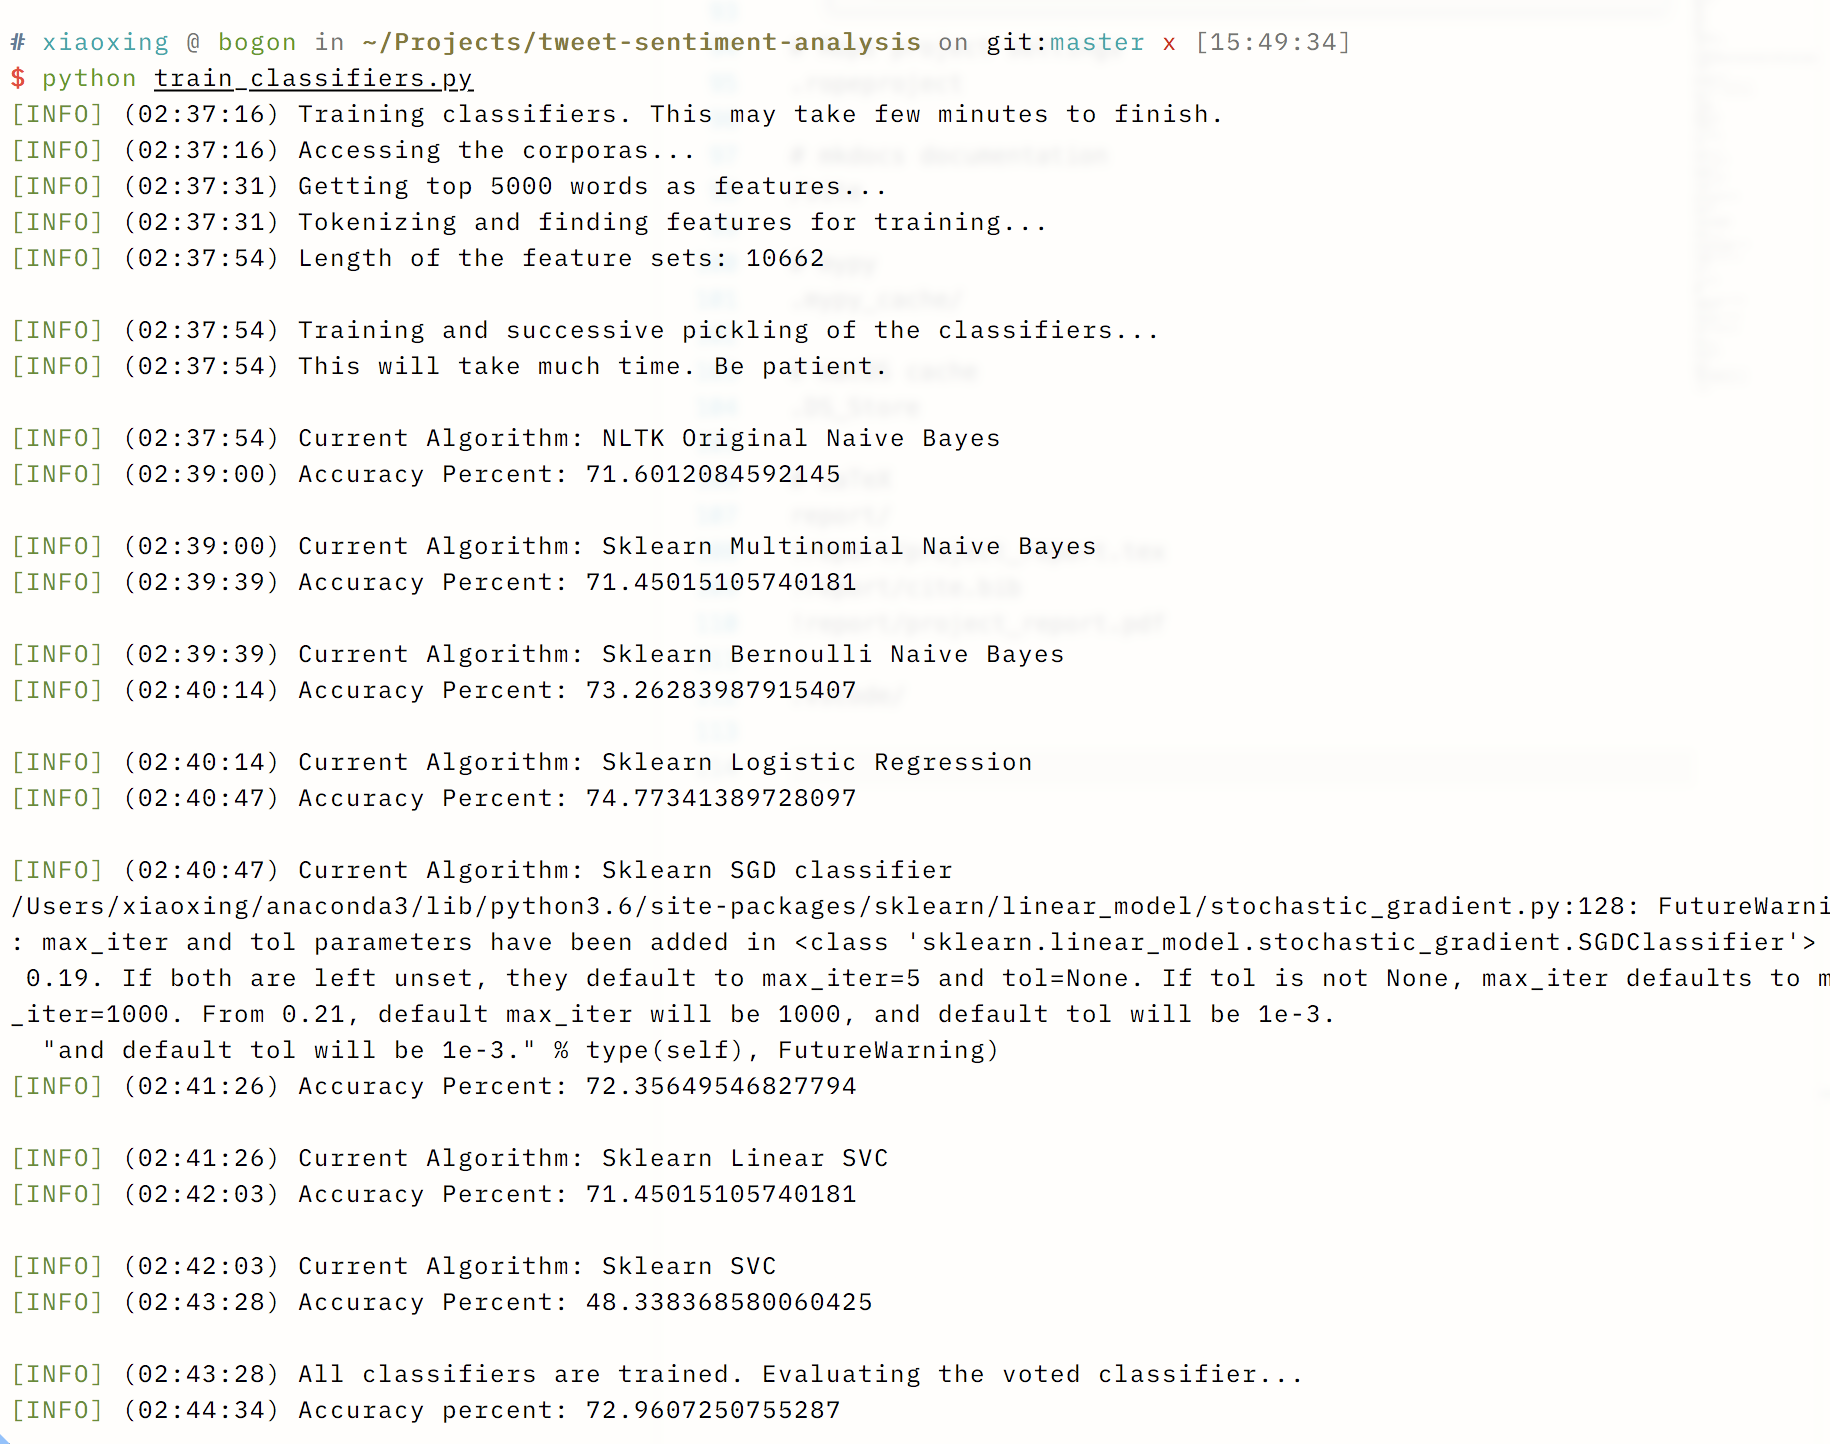
\includegraphics[width=0.9\textwidth]{train_output.png}
      \centering
    \end{figure}

    After we have the trained model, we shall apply the analysis to all tweets we have. Before that, a sentiment analysis function is implemented.

    \inputminted[mathescape, linenos, numbersep=5pt, frame=lines, framesep=2mm, breaklines]{python}{../sentiment.py}

    Then, use a multi-processing technique sentiment_calculation_multithread.py to apply to all rows.

    \inputminted[mathescape, linenos, numbersep=5pt, frame=lines, framesep=2mm, breaklines]{python}{../sentiment_calculation_multithread.py}

  \subsection{Accuracy}
    The accuracy varies because we randomly our training sets. But it should be stable at around $[65, 75]$. This is a demo run:

    \begin{itemize}
      \item NLTK Multinomial Naive Bayes: 72.9607250755287
      \item Sklearn Multinomial Naive Bayes: 70.2416918429003
      \item Sklearn Bernoulli Naive Bayes: 72.35649546827794
      \item Sklearn Logistic Regression: 70.69486404833837
      \item Sklearn Linear SVC: 67.97583081570997
      \item Sklearn SGD classifier: 67.06948640483384
      \item Voted Classifier: 71.75226586102718
    \end{itemize}

  \subsection{Analysis}
    After we have the dataset and the sentiment data, we can now do analysis. Since we have limited memory, we need to optimize the usage. Here we mainly convert categorical data into binary numbers, and choose the correct data types (csv_optimize_to_pickle.py).

    \inputminted[mathescape, linenos, numbersep=5pt, frame=lines, framesep=2mm, breaklines]{python}{"../csv_optimize_to_pickle.py"}

    And, run the score_calculation.py. This will do two parts, one convert the sentiment data into a score ranged from -1 to 1. If the score is between -1 and 0, it means negative, otherwise, positive. Second is to predict what the tweet is talking about, Trump or Hillary. Here we use a naive method -- we have two preset keywords, one for Trump and another for Hillary. If the whole tweet is talking about Trump (no Hillary keyword appear), then the score will be multiplied by -1, while about Hillary by 1. We assume that negative tweets about Trump indicate the positive mind on Hillary, and vice versa. If a tweet is talking about two things, we will then split it into sentenses, and find the most object. After this transformation, the final score will still be ranged from -1 to 1, but now the $[-1, 0)$ part is about Trump, lower then more supportive, and the $(0, 1]$ part is about Hillary, higher then more supportive.

    \inputminted[mathescape, linenos, numbersep=5pt, frame=lines, framesep=2mm, breaklines]{python}{"../score_calculation.py"}

    \begin{figure}[H]
      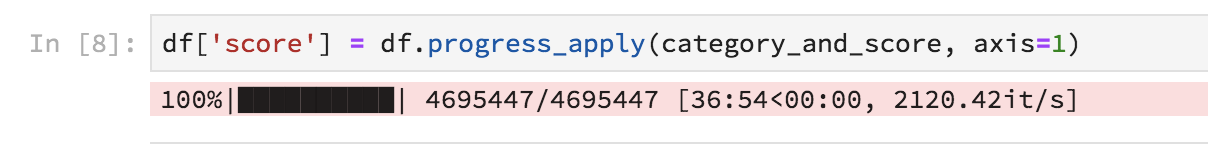
\includegraphics[width=0.9\textwidth]{running.png}
      \centering
    \end{figure}

    Here is some descriptive information on the score distribution.

    \begin{itemize}
      \item For Trump:
            \begin{description}
              \item[count]: 106121.000000
              \item[mean]: -0.915455
              \item[std]: 0.151850
              \item[min]: -1.000000
              \item[25\%]: -1.000000
              \item[50\%]: -1.000000
              \item[75\%]: -0.800000
              \item[max]: -0.033333
            \end{description}
      \item For Hillary:
            \begin{description}
              \item[count]: 196243.000000
              \item[mean]: 0.959576
              \item[std]: 0.111571
              \item[min]: 0.028571
              \item[25\%]: 1.000000
              \item[50\%]: 1.000000
              \item[75\%]: 1.000000
              \item[max]: 1.000000
            \end{description}
    \end{itemize}

    \begin{figure}[H]
      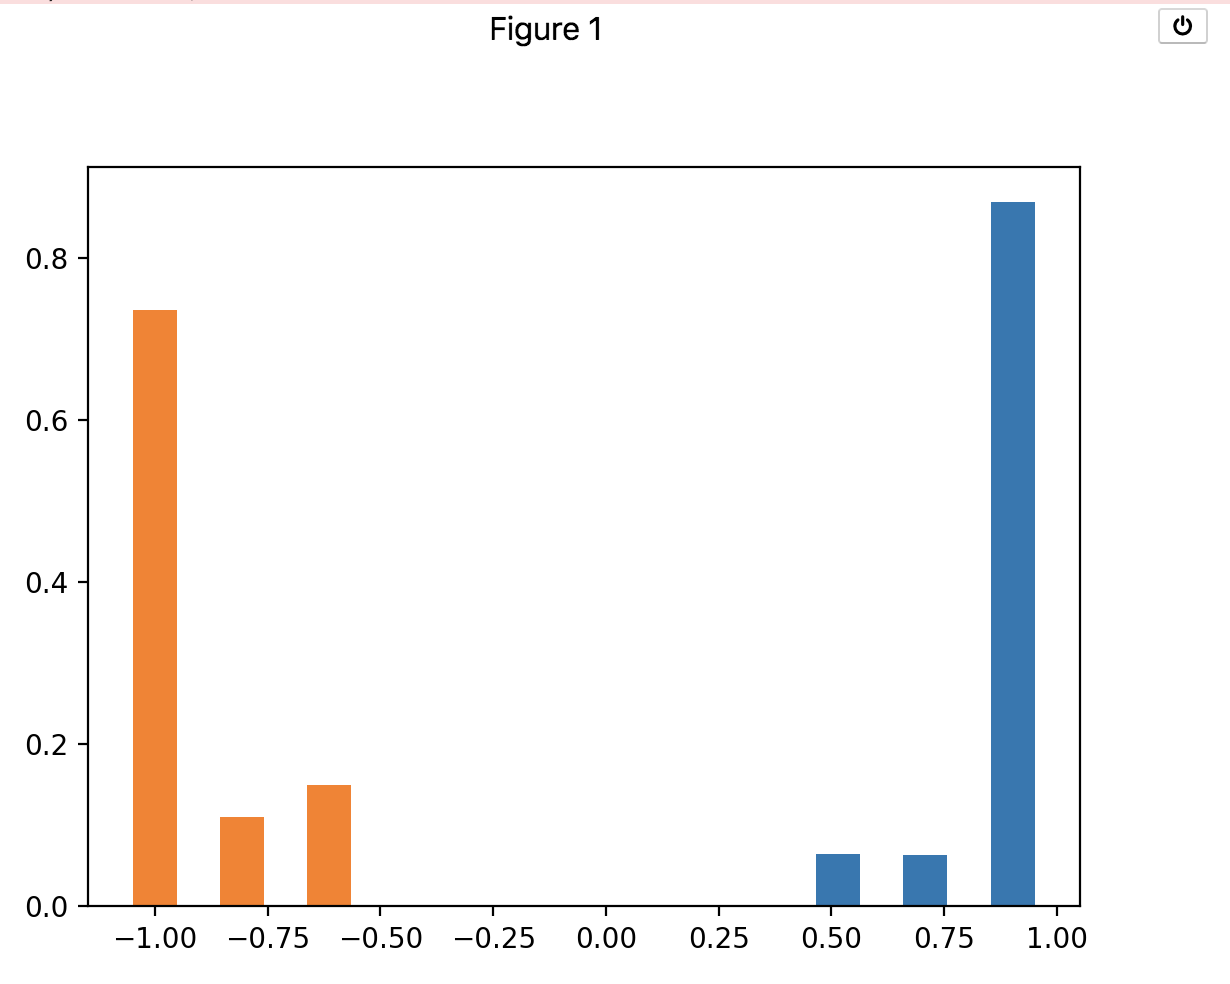
\includegraphics[width=0.9\textwidth]{figure.png}
      \centering
    \end{figure}


\section{Findings and Conclusion}

  As the analysis part (3.4) mentioned, for Trump, the closer the score is to ‘-1’, the more a citizen supporting Trump. Also, the supporting rule is common to Hillary with the score closer to 1. On the result table given in the analysis part (3.4), tweeters for Hillary have a score averaged at 0.959 and Trump have a score averaged at -0.915. Compared Hillary’s score to ‘1’, and Trump’s score to ‘-1’, one can draw the conclusion that from the sentiment data of the tweeter in the day of election, tweeters about Hillary are slightly more positive than tweeters about Trump. Figure 1 shows the clearer score distribution of Trump and Hillary, we can see that the score distribution of Hillary are much closer to 1 compared to the score distribution of Trump to ‘-1’, which indicate the same results of comparing the average score of the two candidates.

  Although the result of tweeter sentiment in this report is different from the real election result, this can be explained by the frequent users of the tweeter. Most people who frequently use tweeter live in the big cities, but in the election, all the states in the United States vote for the president, and not all the people utilize tweeter. Therefore, the prediction by tweeter may contain some bias. However, the close disparity in tweet sentiment is similar to the actual election result, which indicates a connection.

  To further improved the result, having more data from different days may go a step further from the results and improve the accuracy of the prediction. Further study can also be done on the geographical difference of the score. 


  \bibliographystyle{alphadin}
  \bibliography{cite}


\end{document}